\subsection{Legge di Snell}
La Legge di Snell (detta anche Legge della rifrazione) descrive il comportamento della luce (o di un'onda) quando passa da un mezzo a un altro con diverso indice di rifrazione, ovvero spiega quanto e come la luce cambia direzione entrando in un nuovo materiale. La legge si esprime con la formula:
\begin{equation}
	n_1\sin(\theta_1)=n_2\sin(\theta_2)
\end{equation}
dove:
\begin{itemize}
	\item $n_1$ = indice di rifrazione del primo mezzo (da cui parte il raggio),
	\item $n_2$ = indice di rifrazione del secondo mezzo (in cui entra il raggio),
	\item $\theta_1$ = angolo tra il raggio incidente e la normale alla superficie,
	\item $\theta_2$ = angolo tra il raggio rifratto e la normale.
\end{itemize}


\subsection{Funzionamento del prisma di vetro}
Un prisma ottico di vetro è un solido trasparente delimitato da due superfici piane inclinate tra loro (le facce rifrattive) che formano un angolo al vertice $\alpha$. Quando un raggio di luce entra in un prisma, subisce due rifrazioni:

\begin{enumerate}
	\item \textbf{Prima rifrazione:} alla prima faccia di ingresso, quando il raggio passa dall'aria al vetro, deviando verso la normale alla superficie.
	\item \textbf{Seconda rifrazione:} alla seconda faccia, il raggio emerge dal prisma passando dal vetro all'aria, deviando lontano dalla normale.
\end{enumerate}

Queste due deviazioni cumulative producono uno scostamento del raggio emergente rispetto alla direzione originale del raggio incidente. L'effetto complessivo si chiama \textbf{deviazione angolare}.

\begin{figure}[H]
	\centering
	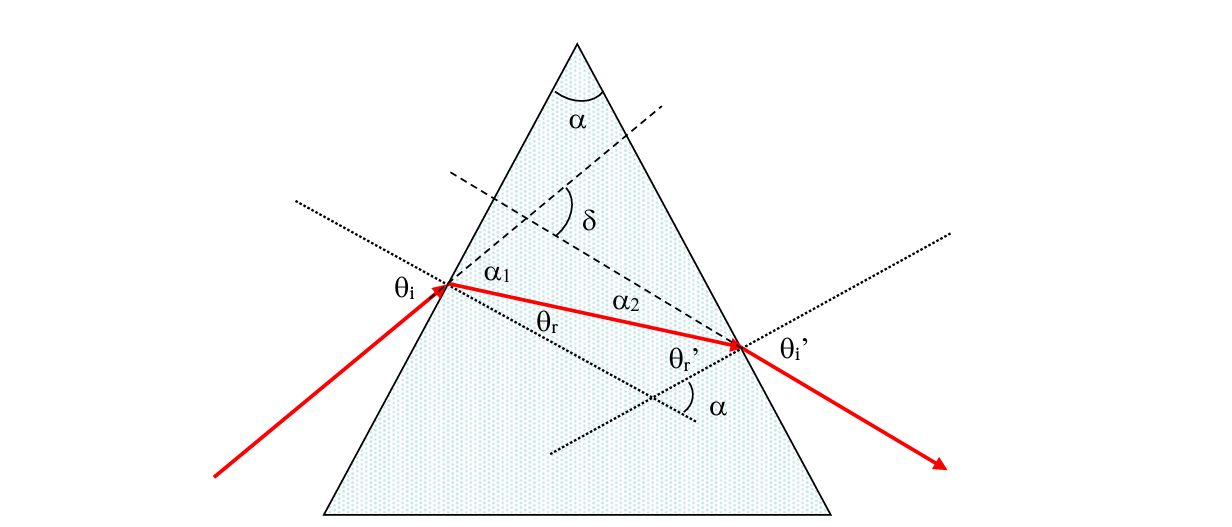
\includegraphics[width=0.75\textwidth]{./figures/prismateoria}
	\caption{Indichiamo: \\
		$\theta_i$ = angolo di incidenza sulla prima faccia (rispetto alla normale) \\
		$\theta_r$ = angolo di rifrazione dentro il prisma sulla prima faccia \\
		$\theta_r'$ = angolo interno di incidenza sulla seconda faccia \\
		$\theta_i'$ = angolo di rifrazione fuori dal prisma (angolo di uscita)}
\end{figure}

Applicando la \textbf{Legge di Snell} alla prima rifrazione:
\begin{equation}
	n_{aria}\sin(\theta_i)=n_{vetro}\sin(\theta_r)
\end{equation}
Poiché $n_aria \approx 1$, si può semplificare:
\begin{equation}
	\sin(\theta_i)=n\sin(\theta_r)
\end{equation}
Dopo il passaggio attraverso il prisma, usando la geometria interna si trova che:
\begin{equation}
	\theta_r'=\alpha-\theta_r
\end{equation}
Applicando ancora la Legge di Snell all'uscita:
\begin{equation}
	n_{vetro}\sin(\theta_r')=n_{aria}\sin(\theta_i') \rightarrow n=\frac{\sin(\theta_i')}{\sin(\theta_r')}
\end{equation}

La deviazione totale $\delta$ è data dalla differenza angolare tra il prolungamento del raggio incidente e il raggio emergente. La formula generale è data dalla Legge (1). Se si cambia lentamente l'angolo di incidenza, l'angolo di deviazione $\delta$ dapprima diminuisce, raggiunge un valore minimo, poi ricomincia ad aumentare. In corrispondenza della deviazione minima $\delta_{min}$ accade che il percorso della luce dentro il prisma è simmetrico: $\theta_i$ e $\theta_i'$ sono uguali, così come $\theta_r$ e $\theta_r'$. In questa situazione:
\begin{equation}
	\theta_r = \theta_r'=\frac{\alpha}{2}
\end{equation}
e si può ricavare l'indice di rifrazione $n$ direttamente con una formula semplice:
\begin{equation}
	n=\frac{\sin\left(\frac{\alpha+\delta_{min}}{2}\right)}{\sin\left(\frac{\alpha}{2}\right)}
\end{equation}
e, tenendo conto dell'uguaglianza $\theta_i=\theta_i'$ e della Legge (1), otteniamo la Legge (2).


\subsection{Richiami Statistici}
Il metodo dei minimi quadrati è una tecnica che permette di trovare una funzione, rappresentata da una curva di regressione, che si avvicini il più possibile ad un insieme di dati (tipicamente punti del piano). In particolare, la funzione trovata deve essere quella che minimizza la somma dei quadrati delle distanze tra i dati osservati e quelli della curva che rappresenta la funzione stessa. Siano $b$ il coefficiente angolare e $a$ l'intercetta della retta di regressione:
\begin{equation}
	b=\frac{\displaystyle\sum_{i=1}^{N}[(x_i-\overline{x})(y_i-\overline{y})]}{\displaystyle\sum_{i=1}^{N}(x_i-\overline{x})^2}
\end{equation}
\begin{equation}
	a=\overline{y}-b\overline{x}
\end{equation}
Con $\overline{x}=\frac{\displaystyle\sum_{i=1}^{N}x_i}{N}$ e $\overline{y}=\frac{\displaystyle\sum_{i=1}^{N}y_i}{N}$
mentre le incertezze:
\begin{equation}
	\Delta b=3\sigma_b
\end{equation}
\begin{equation}
	\Delta a=3\sigma_a
\end{equation}
Con $$\sigma_b=\sigma_y\sqrt{\frac{N}{\Delta}}$$
$$\sigma_y=\sqrt{\frac{\displaystyle\sum_{i=1}^{N}(y_i-bx_i-a)^2}{N-2}}$$
$$\sigma_a=\sigma_y\sqrt{\frac{\displaystyle\sum_{i=1}^{N}x_i^2}{\Delta}}$$
$$\Delta=N\displaystyle\sum_{i=1}^{N}(x_i-\overline{x})^2$$

\subsection{Richiami di teoria della misura}
Sia $g$ una grandezza fisica dipendente da $N$ grandezze fisiche $x_1,...,x_N$ tale che
\begin{equation}
	g=f(x_1,...,x_N)
\end{equation}
con
\begin{equation}
	x_1 = x_{1_0}\pm \Delta x_1
\end{equation}
$$ ... $$
\begin{equation}
	x_N = x_{N_0}\pm \Delta x_N
\end{equation}
La formula di propagazione dell'errore massimo è:
\begin{equation}
	\Delta g=\displaystyle\sum_{i=1}^{N}\left|\frac{\partial g}{\partial x_i}\right|_{\vec{x}=\vec{x_0}}\Delta x_i
\end{equation}
con
\begin{equation}
	\vec{x}=(x_1,...,x_N)
\end{equation}
\begin{equation}
	\vec{x_0}=(x_{1_0},...,x_{N_0})
\end{equation}
Sia g una grandezza fisica pari alla somma, o alla differenza, di N grandezze fisiche $x_1,...,x_N$ tale che
\begin{equation}
	g=x_1\pm...\pm x_N
\end{equation}
con
\begin{equation}
	x_1=x_{1_0}\pm \Delta x_N
\end{equation}
$$ ... $$
\begin{equation}
	x_N=x_{N_0}\pm \Delta x_N
\end{equation}
La formula di propagazione dell'errore massimo è:
\begin{equation}
	\Delta g= \Delta x_1+...+\Delta x_N
\end{equation}

